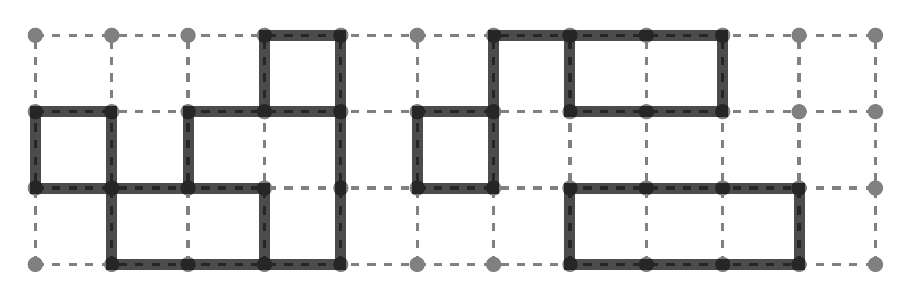
\begin{tikzpicture}[scale=0.97]
  \draw[very thick, gray, dashed] (0,0) grid (11,3);
  \foreach \i in {0,1,2,3} {
    \foreach \j in {0,1,2,3,4,5,6,7,8,9,10,11} {
      \fill[gray] (\j, \i) circle (0.1);
    }
  }
  \draw[line width=4, opacity=0.7]
    (3,0)--(3,1)--(0,1)--(0,2)--(1,2)--(1,0)--(4,0)--(4,3)--(3,3)--(3,2)--(4,2)
    (2,1)--(2,2)--(3,2)

    (6,2)--(5,2)--(5,1)--(6,1)--(6,2)--(6,3)--(7,3)--(8,3)--(9,3)--(9,2)--(8,2)--(7,2)--(7,3)
    (10,0)--(10,1)--(7,1)--(7,0)--cycle
  ;
\end{tikzpicture}
